\documentclass{ximera}
\usepackage{sagetex}
\usepackage{multicol}
%% handout
%% space
%% newpage
%% numbers
%% nooutcomes

%% You can put user macros here
%% However, you cannot make new environments

\graphicspath{{./}{module1Activity/}{module2Activity/}{module3Activity/}}

\usepackage{sagetex}
\usepackage{tikz}
\usepackage{hyperref}
\usepackage{tkz-euclide}
\usetkzobj{all}
\pgfplotsset{compat=1.7} % prevents compile error.

\tikzstyle geometryDiagrams=[ultra thick,color=blue!50!black]
 %% we can turn off input when making a master document

\outcome{Understand and solve quadratic equations.}
\author{Darryl Chamberlain Jr.}
 
\title{Objective 2 - Graphing quadratic functions.}

\begin{document}
\begin{abstract}
Describe the salient characteristics of quadratic functions.
\end{abstract}
\maketitle

\href{https://cnx.org/contents/mwjClAV_@8.1:-Sm9he1Q@17/Quadratic-Functions}{Link to section in online textbook.}

%%%%%%%%%%%%%%%%%%%%%
%%%  Objective 1  %%%
%%%%%%%%%%%%%%%%%%%%%

First, watch 
\href{https://mediasite.video.ufl.edu/Mediasite/Play/b3664c4b8bbb458a969fecac7a80759c1d}{this video} to review the main characteristics of a quadratic function. Feel free to pause the video and fill out the notes as you go. 

Now practice working with converting between quadratic equations and their graphs below. 

\begin{question}
Write the equation of the graph presented below in the form $f(x)=ax^2+bx+c$, assuming $a=1$ or $a=-1$. 

\begin{center}
	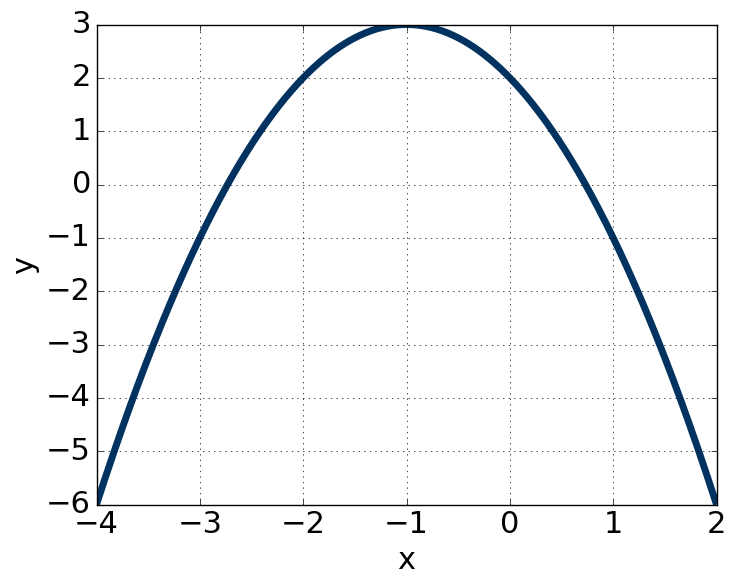
\includegraphics[width = 0.4\textwidth]{question1Astatic.png}
\end{center}
% $-(x+1)^2+3 = -(x^2+2x+1)+3 = -x^2-2x+2 $
$y = \answer{-1} x^2 + \answer{-2} x + \answer{2}$
\end{question}

\begin{question}
Write the equation of the graph presented below in the form $f(x)=ax^2+bx+c$, assuming $a=1$ or $a=-1$. 

\begin{center}
	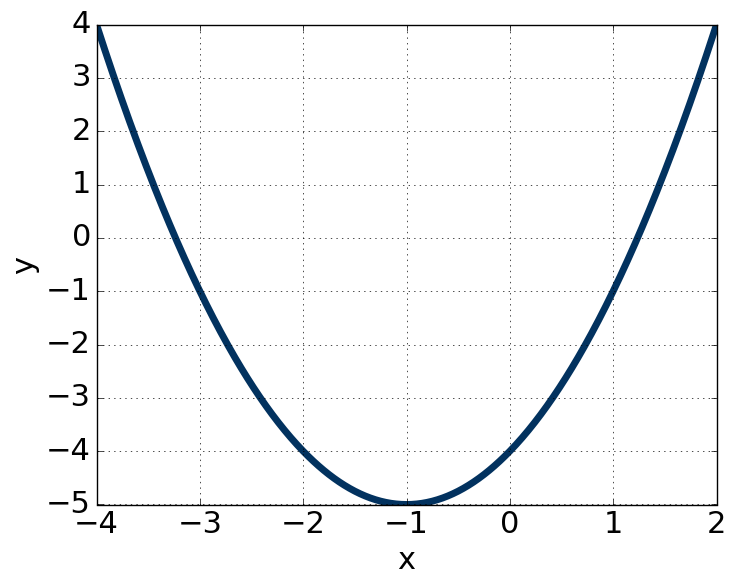
\includegraphics[width = 0.4\textwidth]{question1Bstatic.png}
\end{center}

% $(x+1)^2-5 = x^2+2x+1-5=x^2+2x-4 $
$y = \answer{1} x^2 + \answer{2} x + \answer{-4}$
\end{question}

\begin{question}
Write the equation of the graph presented below in the form $f(x)=ax^2+bx+c$, assuming $a=1$ or $a=-1$. 

\begin{center}
	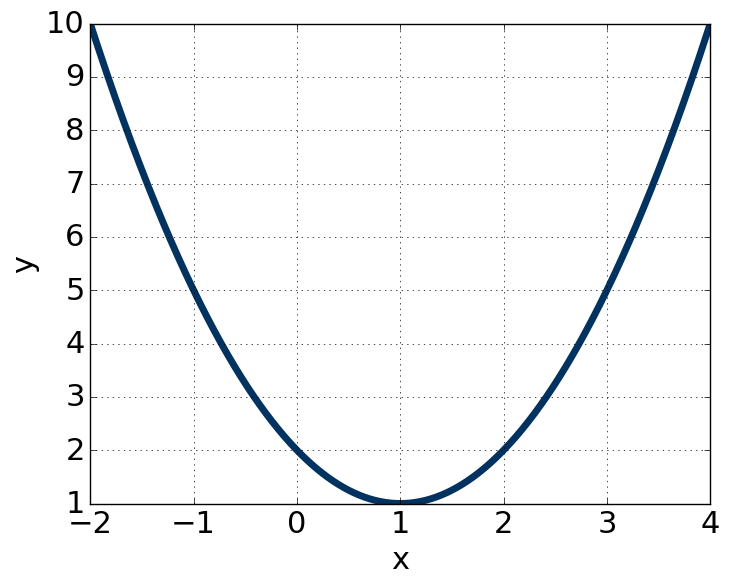
\includegraphics[width = 0.4\textwidth]{question1Cstatic.png}
\end{center}

$y = \answer{1} x^2 + \answer{-2} x + \answer{2}$
\end{question}

\begin{question}
Graph the equation $f(x)= (x-3)^2-19. $

\begin{table}
\begin{tabular}{l l}
	\begin{tabular}{|c c|}
		\hline 
		& \\
		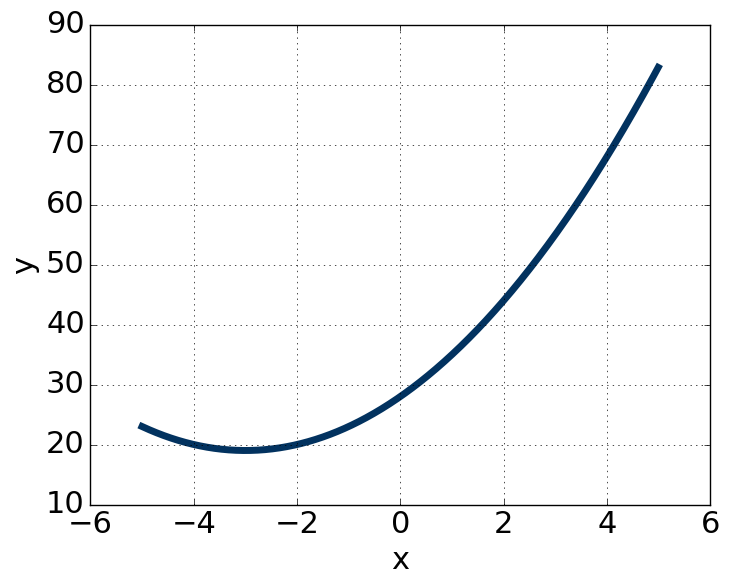
\includegraphics[width = 0.3\textwidth]{question2Astatic.png} & Choice A \\   & \\ 
		\hline
		& \\
		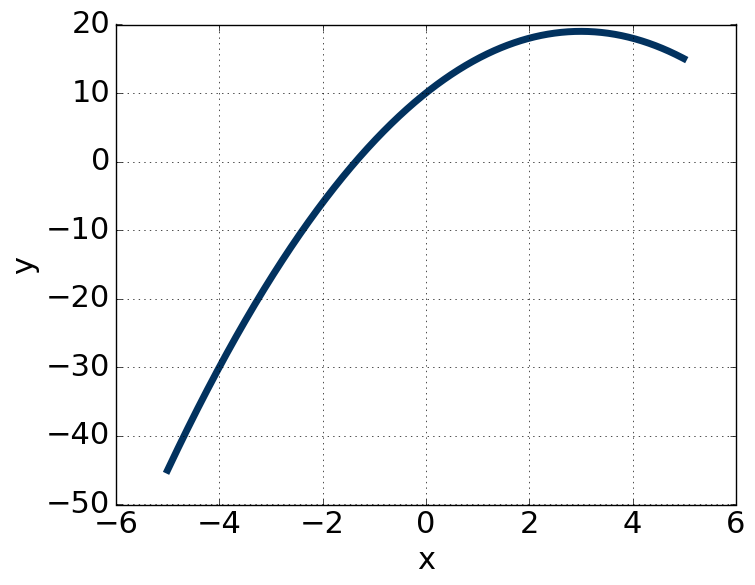
\includegraphics[width = 0.3\textwidth]{question2Bstatic.png} & Choice B \\
		& \\
		\hline 
		& \\
		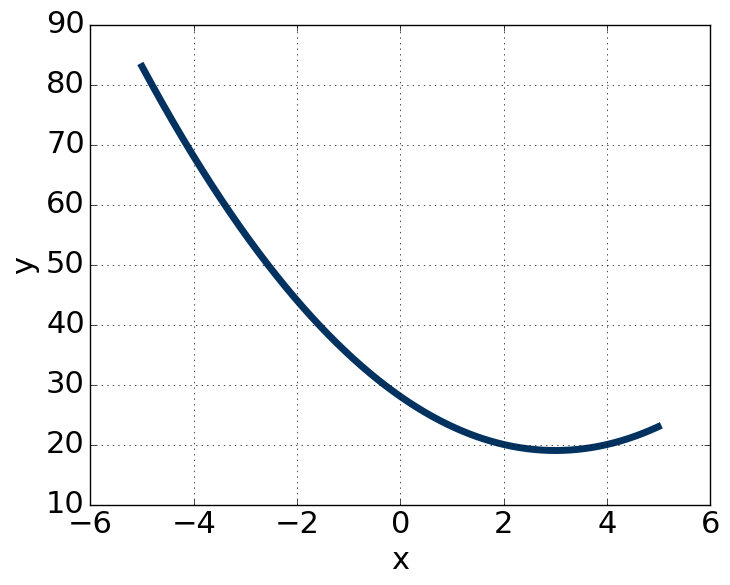
\includegraphics[width = 0.3\textwidth]{question2Cstatic.png} & Choice C \\
		& \\
		\hline 
	\end{tabular}

	\begin{tabular}{|c c|}
		\hline
		& \\
		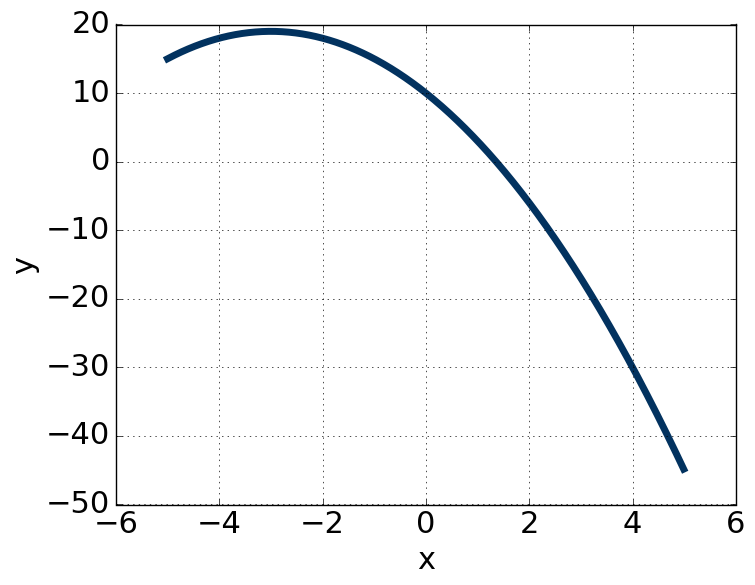
\includegraphics[width = 0.3\textwidth]{question2Dstatic.png} & Choice D \\
		& \\
		\hline 
		& \\
		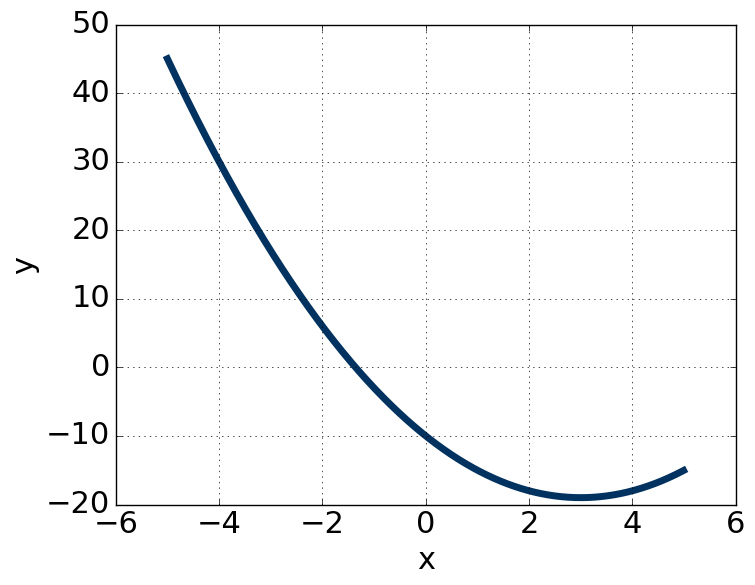
\includegraphics[width = 0.3\textwidth]{question2Estatic.png} & Choice E \\
		& \\
		\hline 
	\end{tabular}
\end{tabular}
\end{table}


\begin{multipleChoice}
    \choice A
    \choice B
    \choice C
    \choice D
    \choice[correct] E
\end{multipleChoice}

\end{question}

\end{document}
